\documentclass{article}
\usepackage[utf8]{inputenc}
\usepackage[spanish]{babel}
\usepackage{geometry}
\usepackage{amssymb}
\usepackage{tikz}
\usepackage{graphicx}
\usetikzlibrary{perspective}
\geometry{letterpaper,margin=2cm} 
\title{Tesis}

\begin{document}

\begin{figure}[h!]
    \centering
    \begin{minipage}{0.45\textwidth}
        \centering
        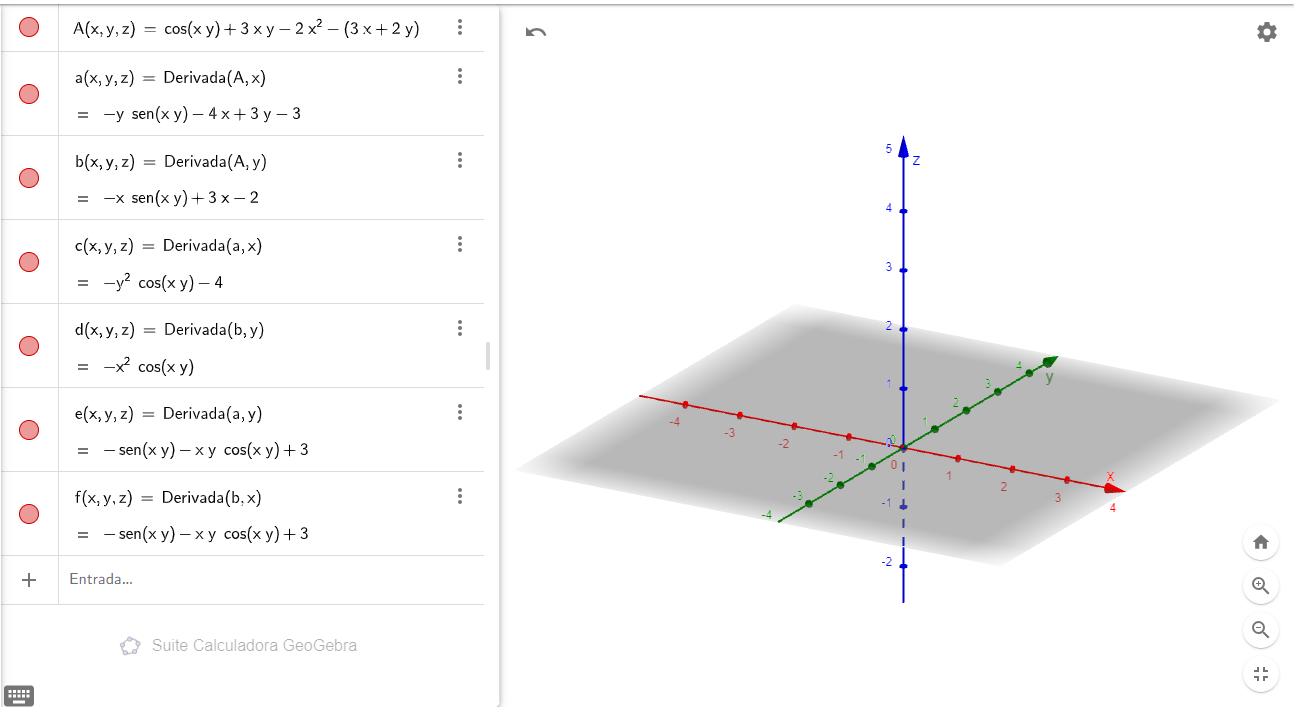
\includegraphics[width=\textwidth]{imgs/derivada_parcial_Geogebra.png}
        \caption*{Izquierda: GeoGebra}
    \end{minipage}
    \hfill
    \begin{minipage}{0.45\textwidth}
        \centering
        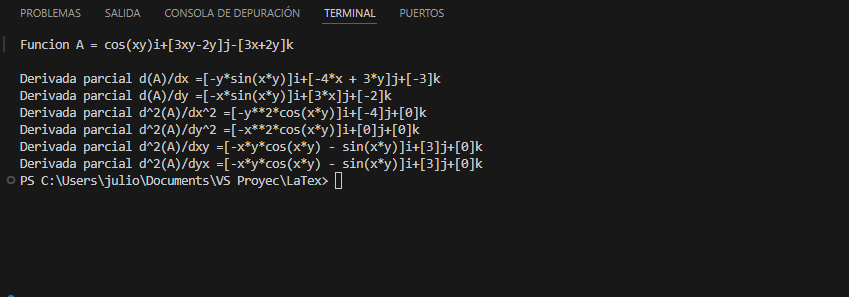
\includegraphics[width=\textwidth]{imgs/derivada_parcial_Python.png}
        \caption*{Derecha: Python}
    \end{minipage}
    
    \vspace{0.5cm}
    
    \begin{minipage}{0.45\textwidth}
        \centering
        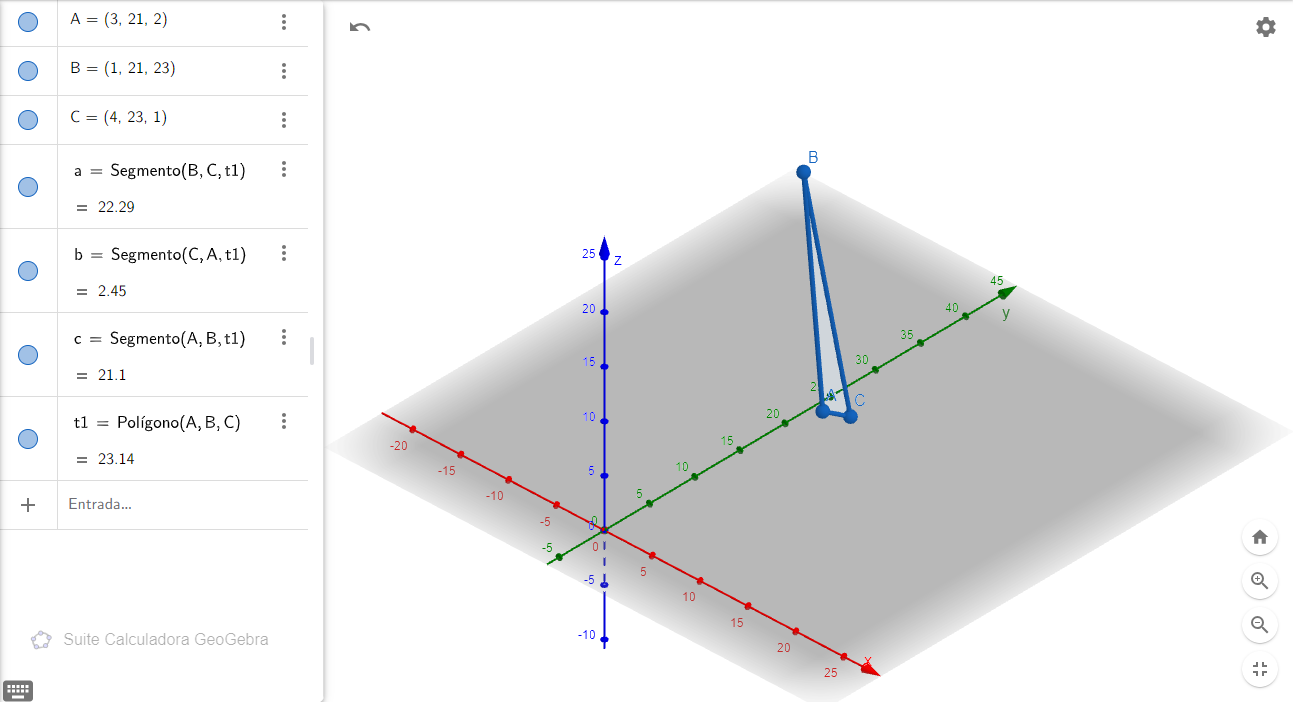
\includegraphics[width=\textwidth]{imgs/triangulo_A_Geogebra.png}
    \end{minipage}
    \hfill
    \begin{minipage}{0.45\textwidth}
        \centering
        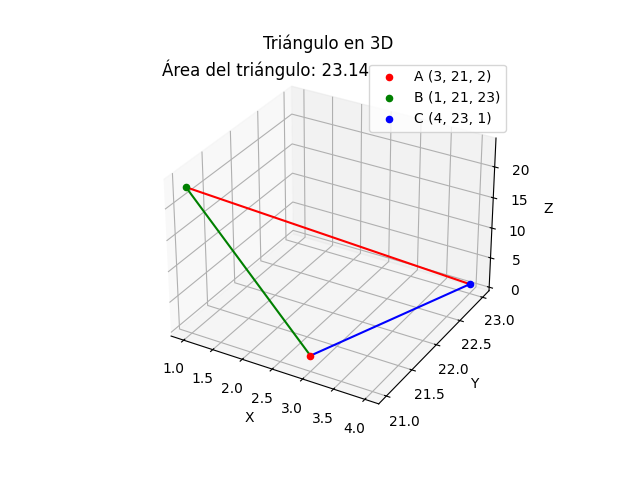
\includegraphics[width=\textwidth]{imgs/triangulo_A_python.png}
    \end{minipage}
    
    \vspace{0.5cm}
    
    \begin{minipage}{0.45\textwidth}
        \centering
        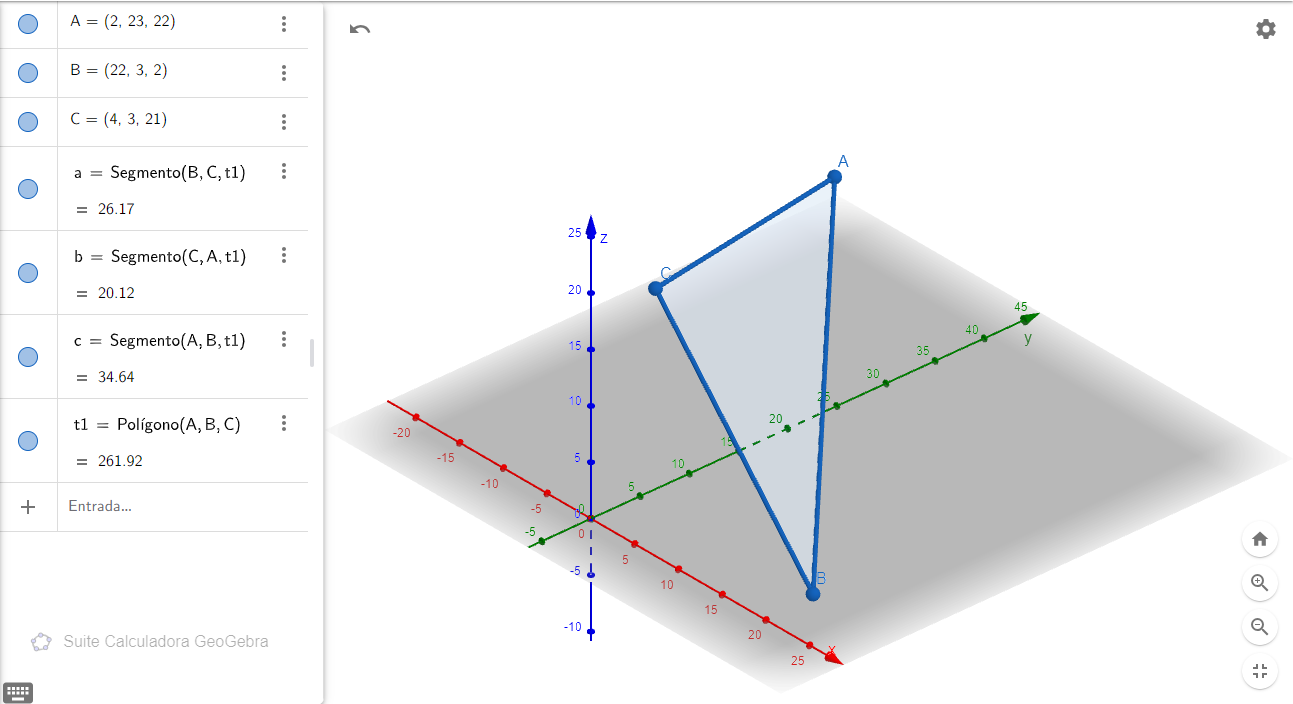
\includegraphics[width=\textwidth]{imgs/triangulo_B_Geogebra.png}
    \end{minipage}
    \hfill
    \begin{minipage}{0.45\textwidth}
        \centering
        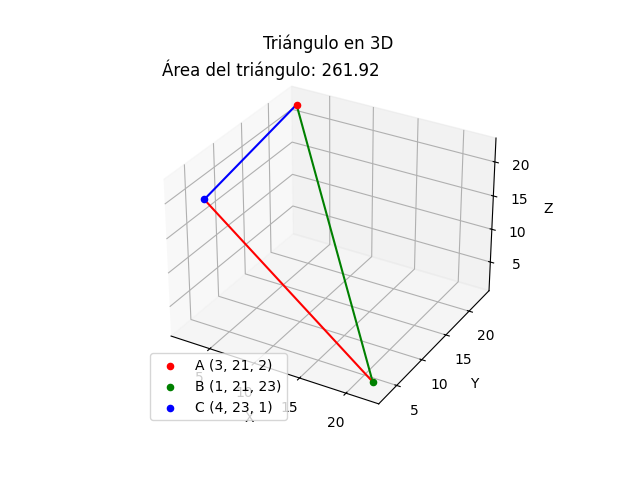
\includegraphics[width=\textwidth]{imgs/triangulo_B_python.png}
    \end{minipage}
    
    \vspace{0.5cm}
    
    \begin{minipage}{0.45\textwidth}
        \centering
        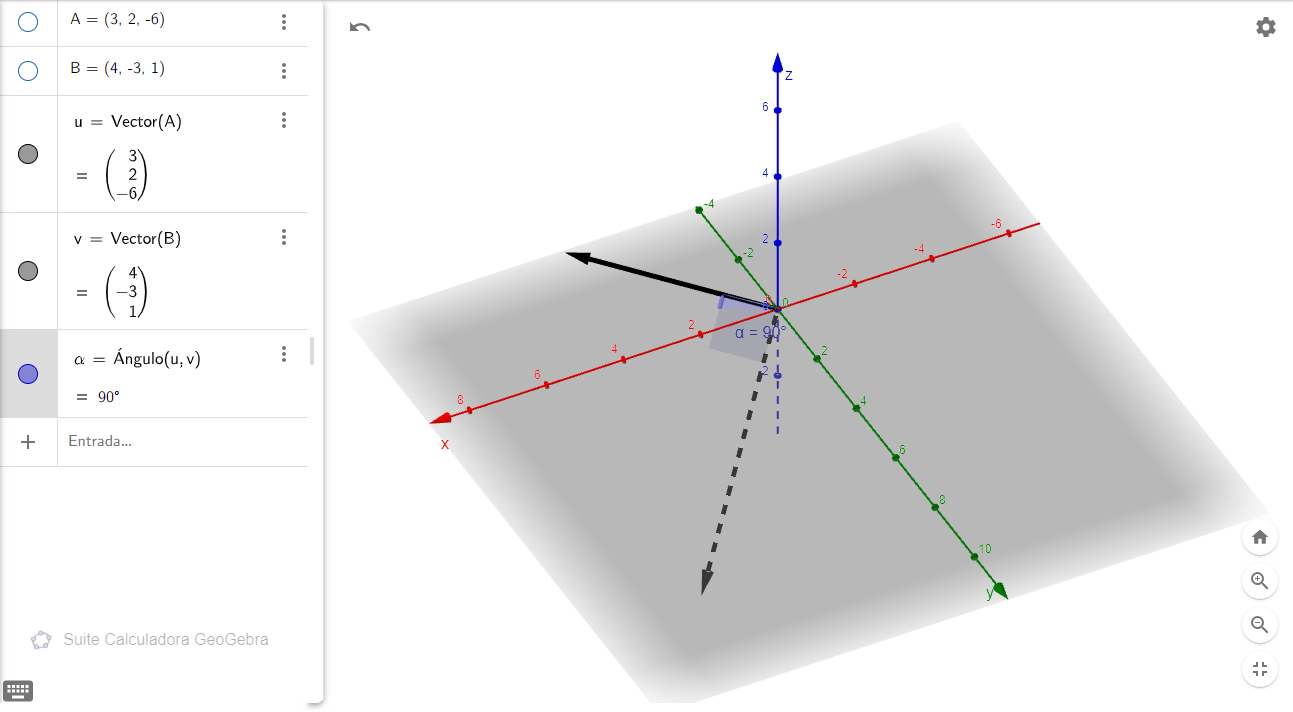
\includegraphics[width=\textwidth]{imgs/vectores_AB_Geogebra.png}
    \end{minipage}
    \hfill
    \begin{minipage}{0.45\textwidth}
        \centering
        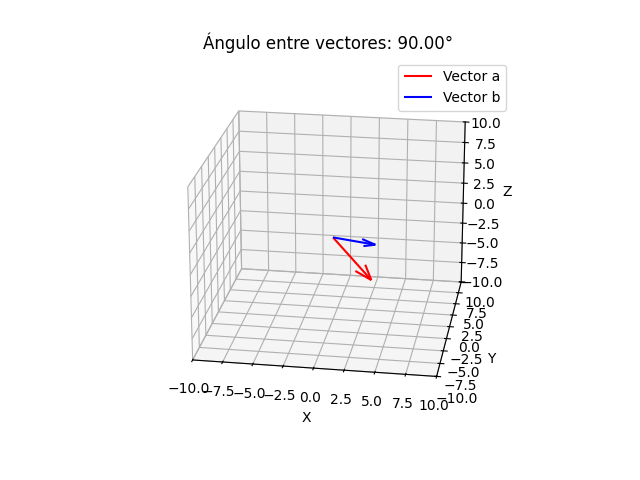
\includegraphics[width=\textwidth]{imgs/vectores_AB_python.png}
    \end{minipage}
    
    \caption{Izquierda imágenes generadas con GeoGebra y a la derecha los resultados en Python}
\end{figure}

\begin{figure}[h!]
    \centering
    \begin{minipage}{0.45\textwidth}
        \centering
        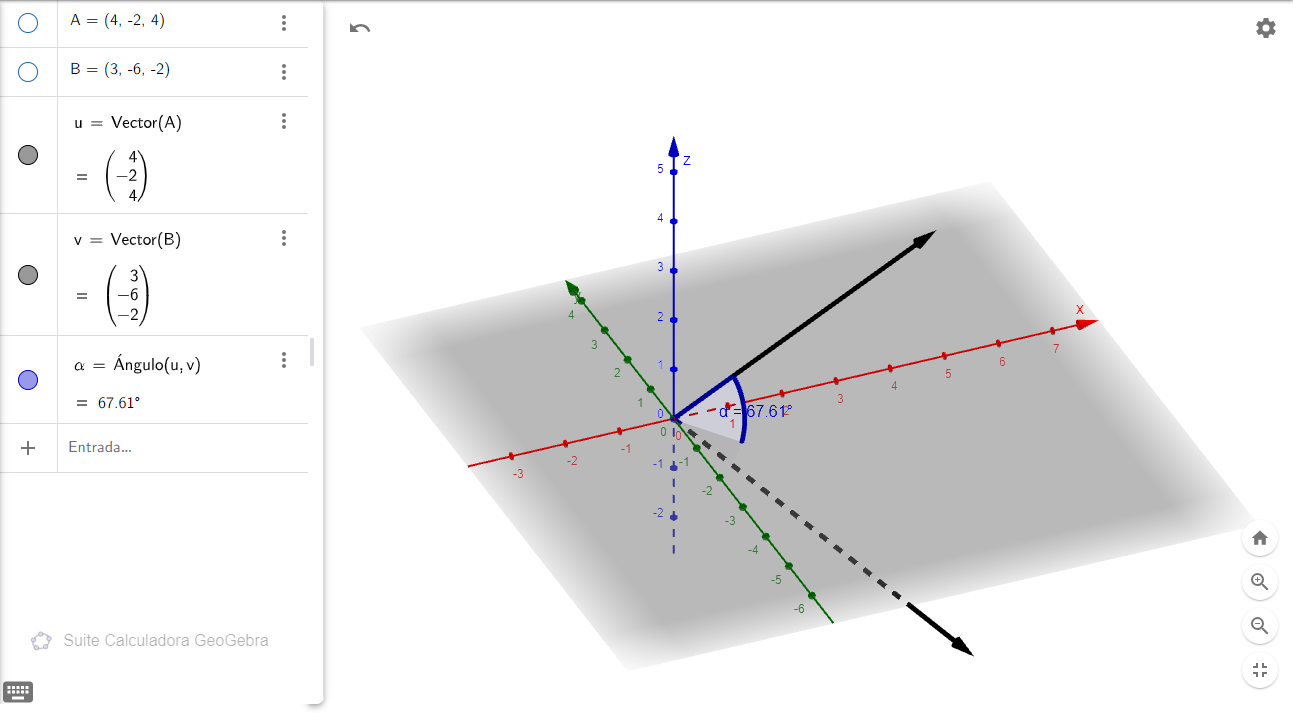
\includegraphics[width=\textwidth]{imgs/vectores_CD_Geogebra.png}
    \end{minipage}
    \hfill
    \begin{minipage}{0.45\textwidth}
        \centering
        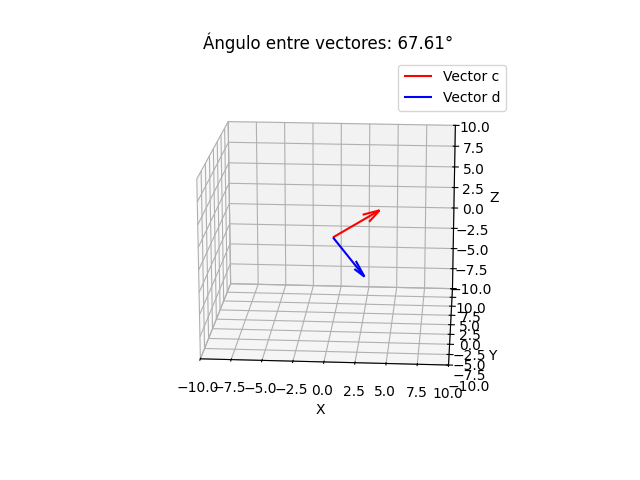
\includegraphics[width=\textwidth]{imgs/vectores_CD_python.png}
    \end{minipage}
    
    \vspace{0.5cm}
    
    \begin{minipage}{0.45\textwidth}
        \centering
        \includegraphics[width=\textwidth]{imgs/ϕ(x,y,z)_A_Geogebra.png}
    \end{minipage}
    \hfill
    \begin{minipage}{0.45\textwidth}
        \centering
        \includegraphics[width=\textwidth]{imgs/ϕ(x,y,z)_A_Python.png}
    \end{minipage}
    
    \vspace{0.5cm}
    
    \begin{minipage}{0.45\textwidth}
        \centering
        \includegraphics[width=\textwidth]{imgs/ϕ(x,y,z)_B_Geogebra.png}
    \end{minipage}
    \hfill
    \begin{minipage}{0.45\textwidth}
        \centering
        \includegraphics[width=\textwidth]{imgs/ϕ(x,y,z)_B_Python.png}
    \end{minipage}
    
    \caption{Izquierda imágenes generadas con GeoGebra y a la derecha los resultados en Python}
\end{figure}

\begin{figure}[h!]
    \centering
    \begin{minipage}{0.45\textwidth}
        \centering
        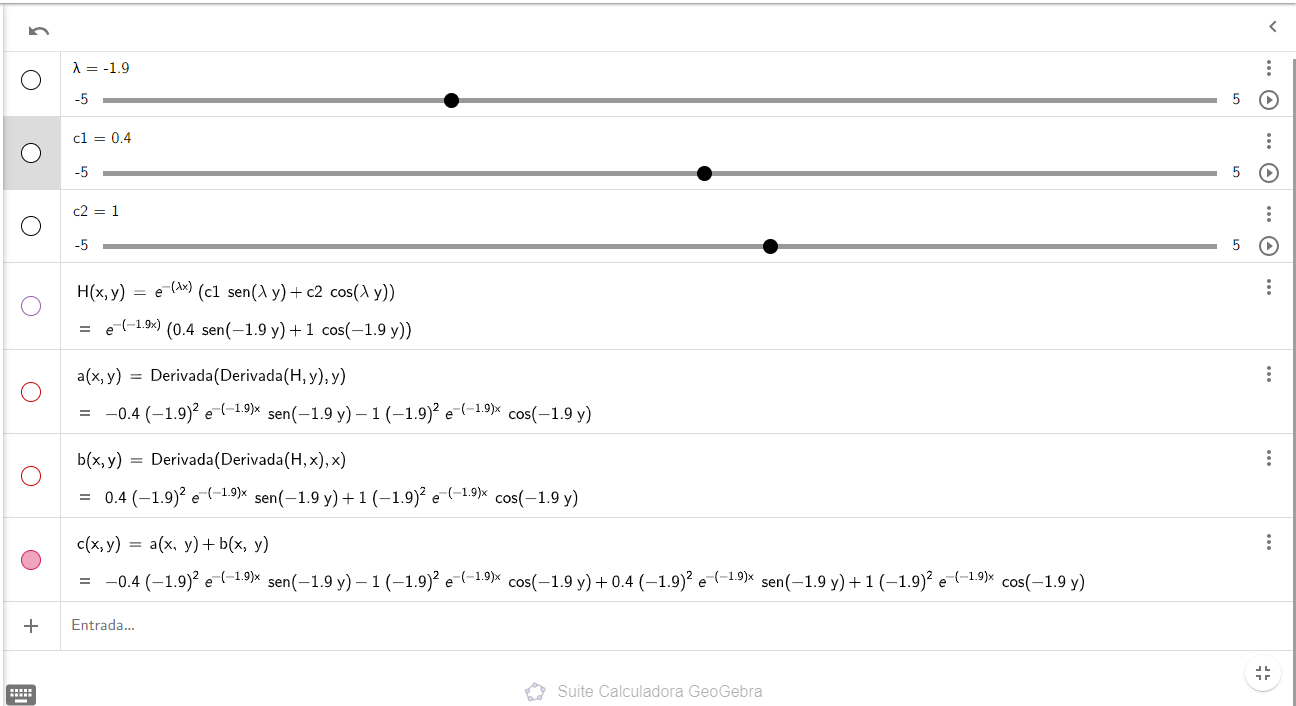
\includegraphics[width=\textwidth]{imgs/derivada_parcial_+_Geogebra.png}
    \end{minipage}
    \hfill
    \begin{minipage}{0.45\textwidth}
        \centering
        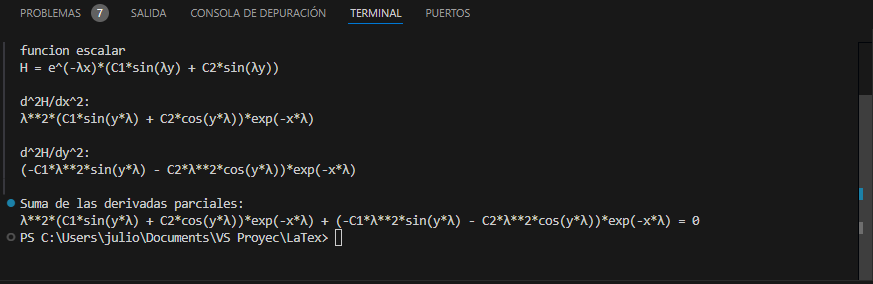
\includegraphics[width=\textwidth]{imgs/derivada_parcial_+_Python.png}
    \end{minipage}
    
    \vspace{0.5cm}
    
    \begin{minipage}{0.45\textwidth}
        \centering
        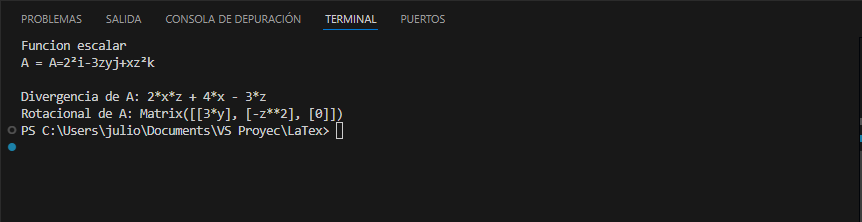
\includegraphics[width=\textwidth]{imgs/Div_Rot_python.png}
    \end{minipage}
    \hfill
    \begin{minipage}{0.45\textwidth}
        \centering
        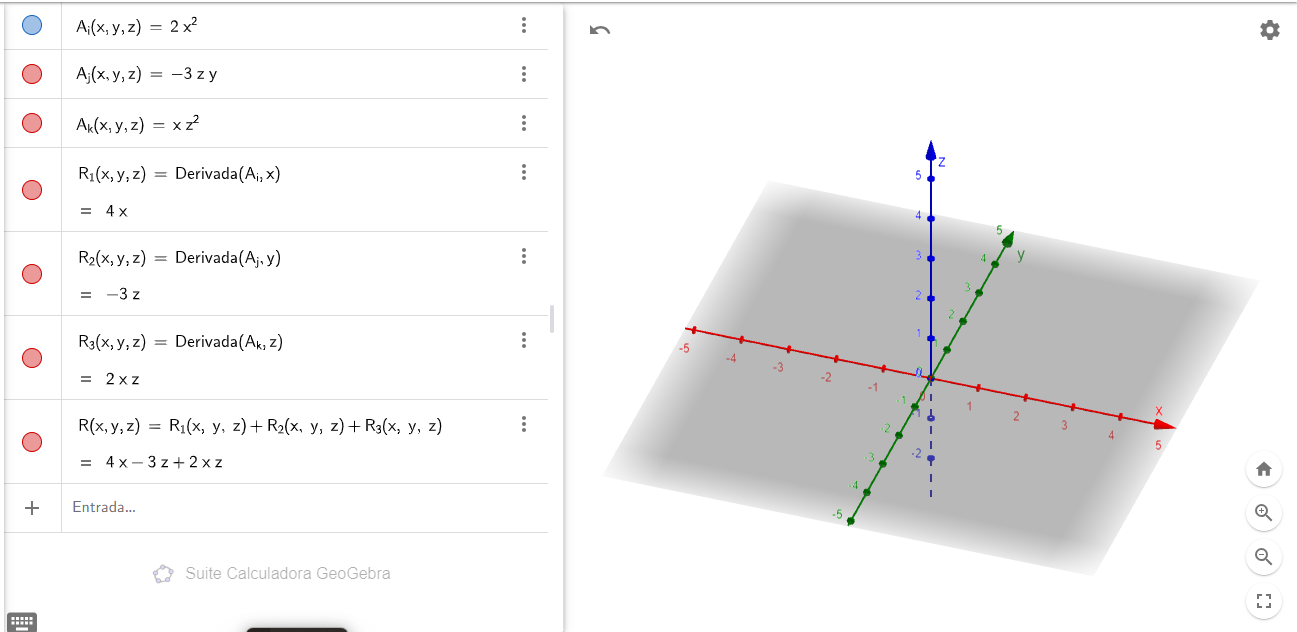
\includegraphics[width=\textwidth]{imgs/divergencia_Geogebra.png}
    \end{minipage}
    
    \vspace{0.5cm}
    
    \begin{minipage}{0.45\textwidth}
        \centering
        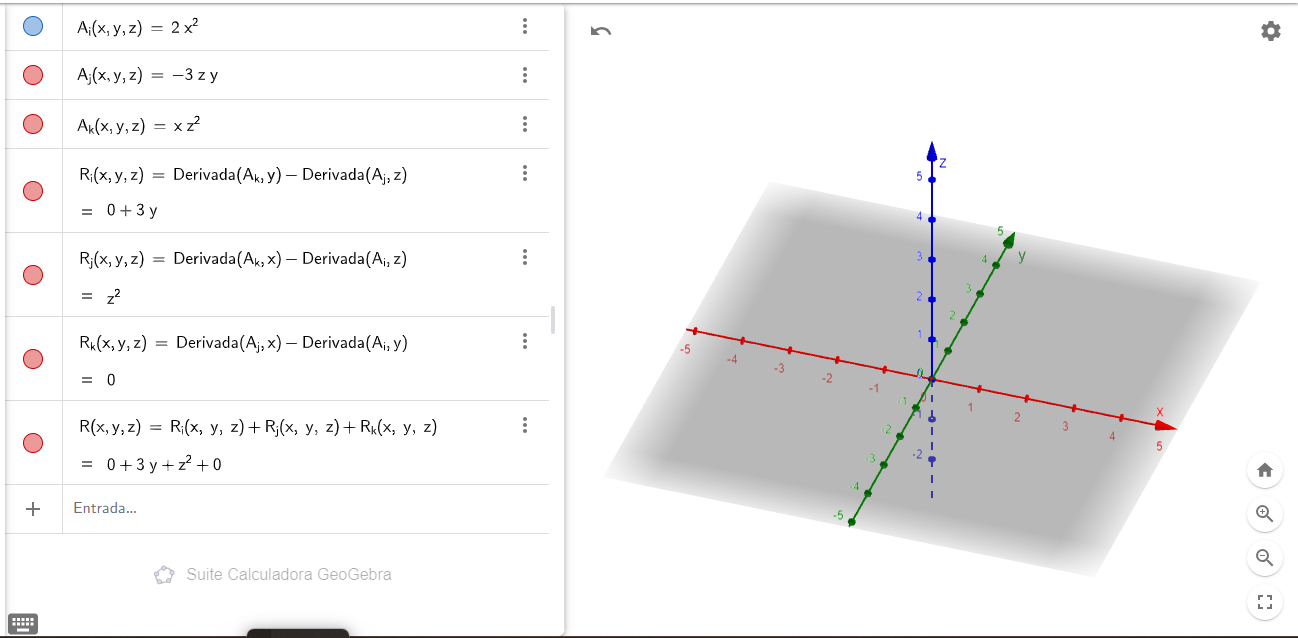
\includegraphics[width=\textwidth]{imgs/Rotacional_Geogebra.png}
    \end{minipage}
    
    \caption{Izquierda imágenes generadas con GeoGebra y a la derecha los resultados en Python}
\end{figure}

\begin{figure}[h!]
    \centering
    \begin{minipage}{0.45\textwidth}
        \centering
        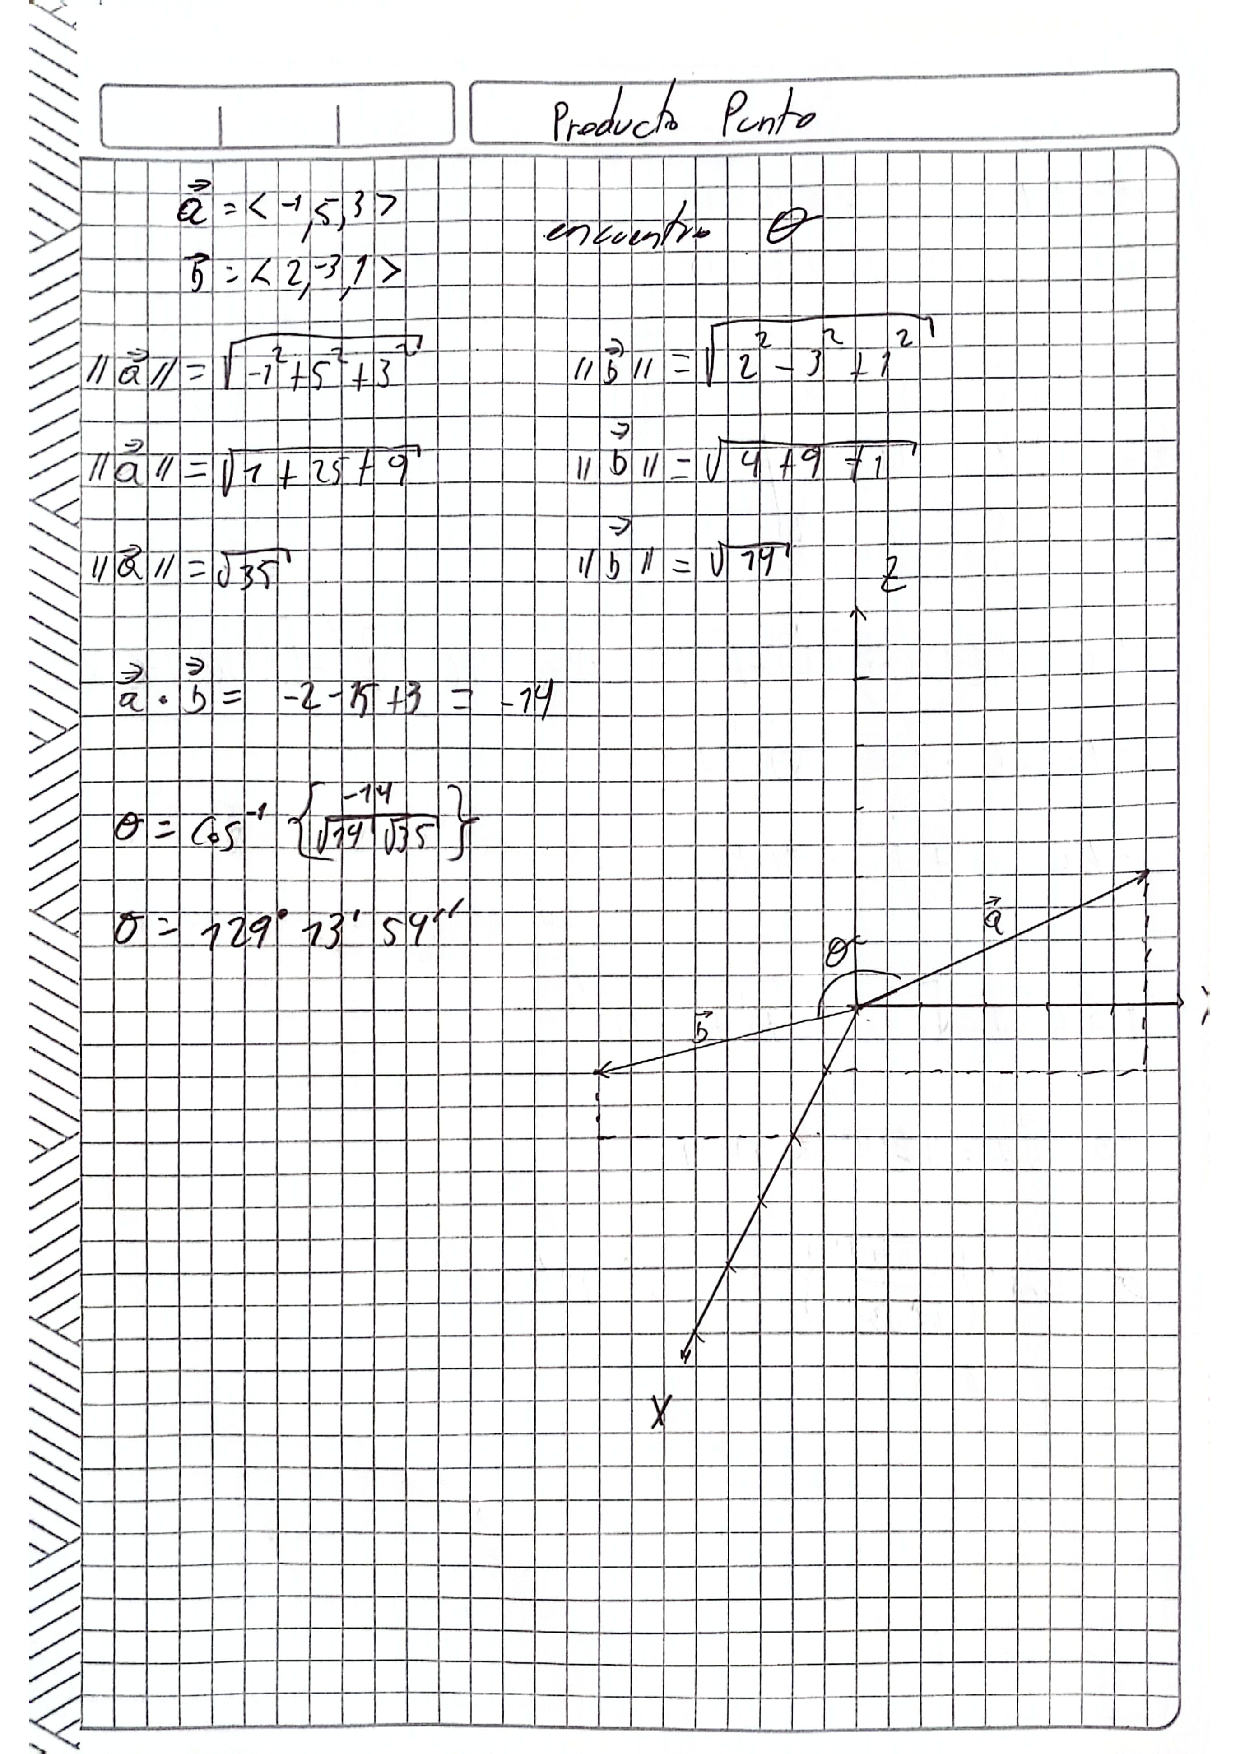
\includegraphics[width=\textwidth]{imgs/Actividad 3 julio amaya.pdf}
    \end{minipage}
    \hfill
    \begin{minipage}{0.45\textwidth}
        \centering
        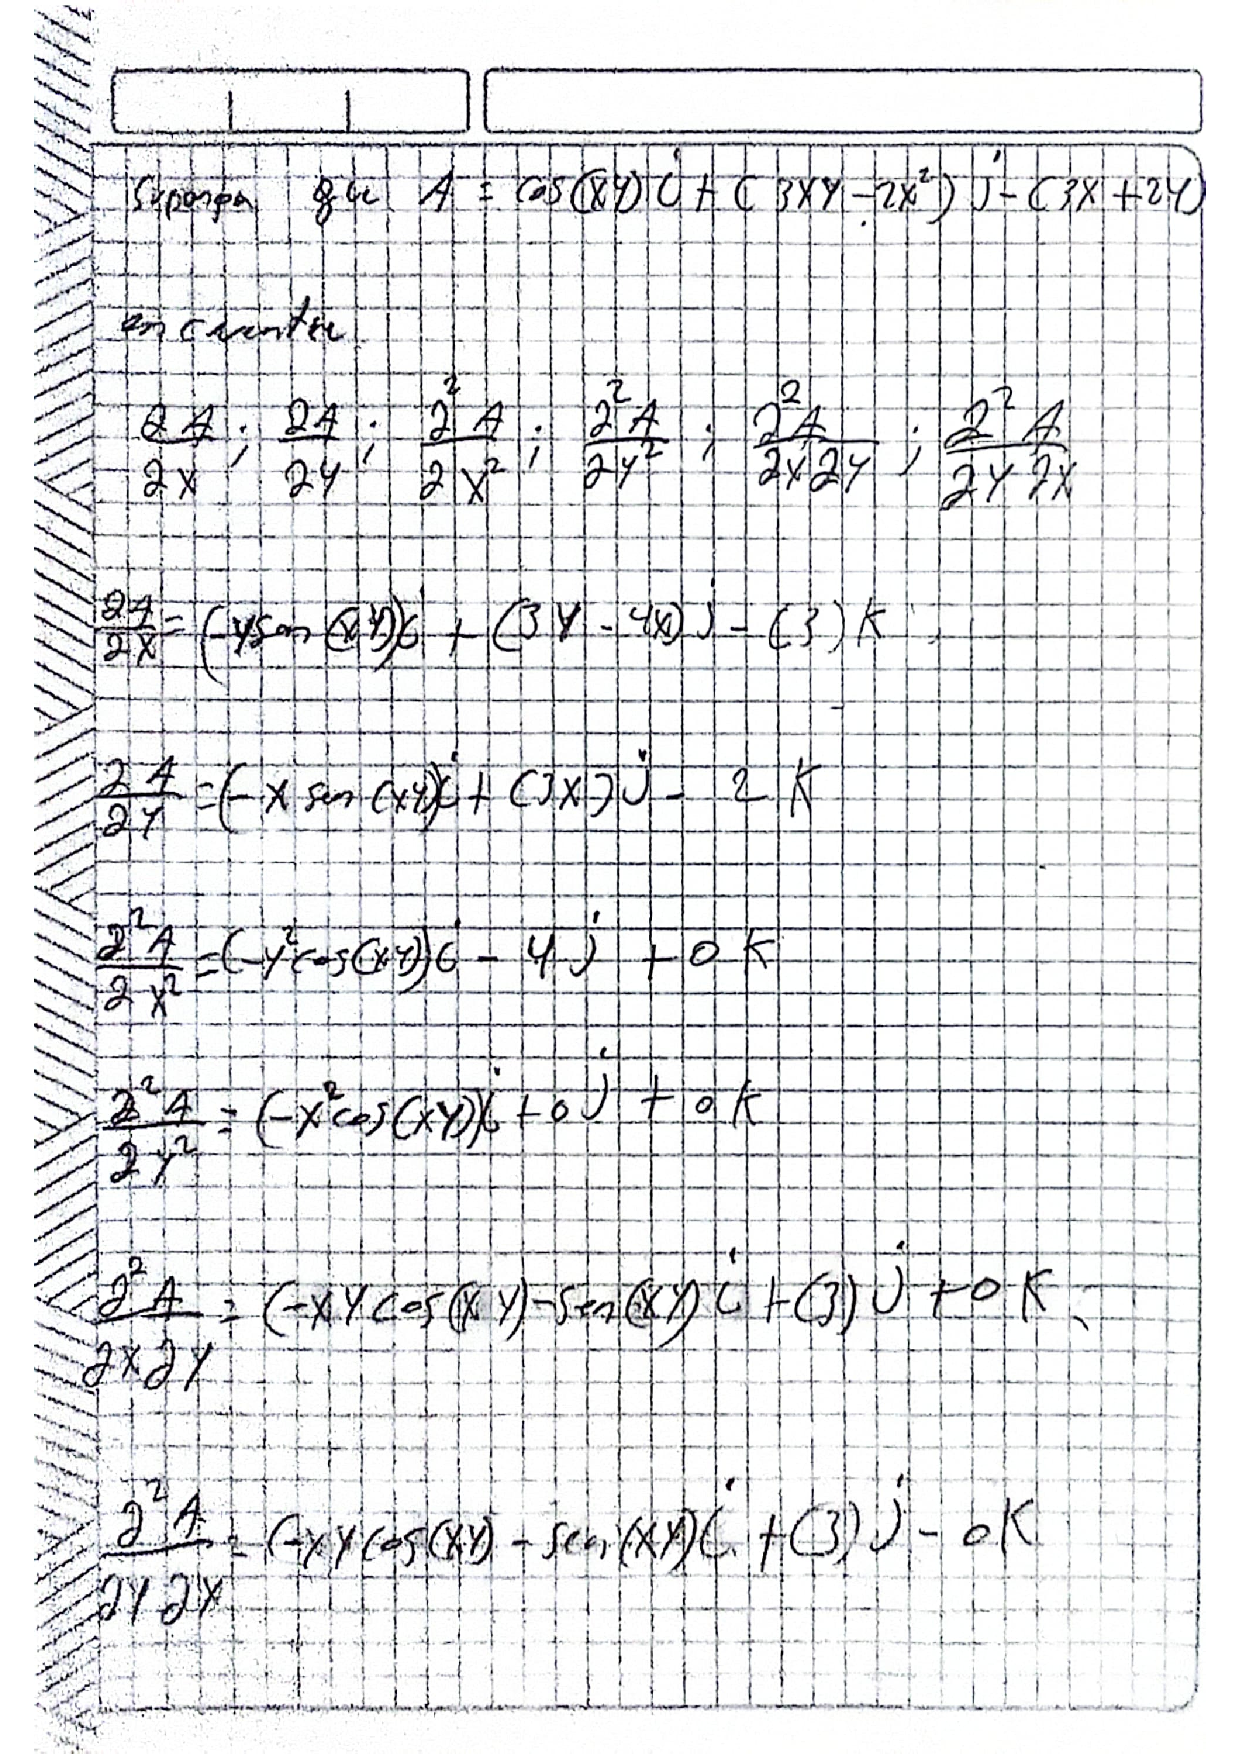
\includegraphics[width=\textwidth]{imgs/Actividad 5 julio amaya.pdf}
    \end{minipage}
    
    \vspace{0.5cm}
    
    \begin{minipage}{0.45\textwidth}
        \centering
        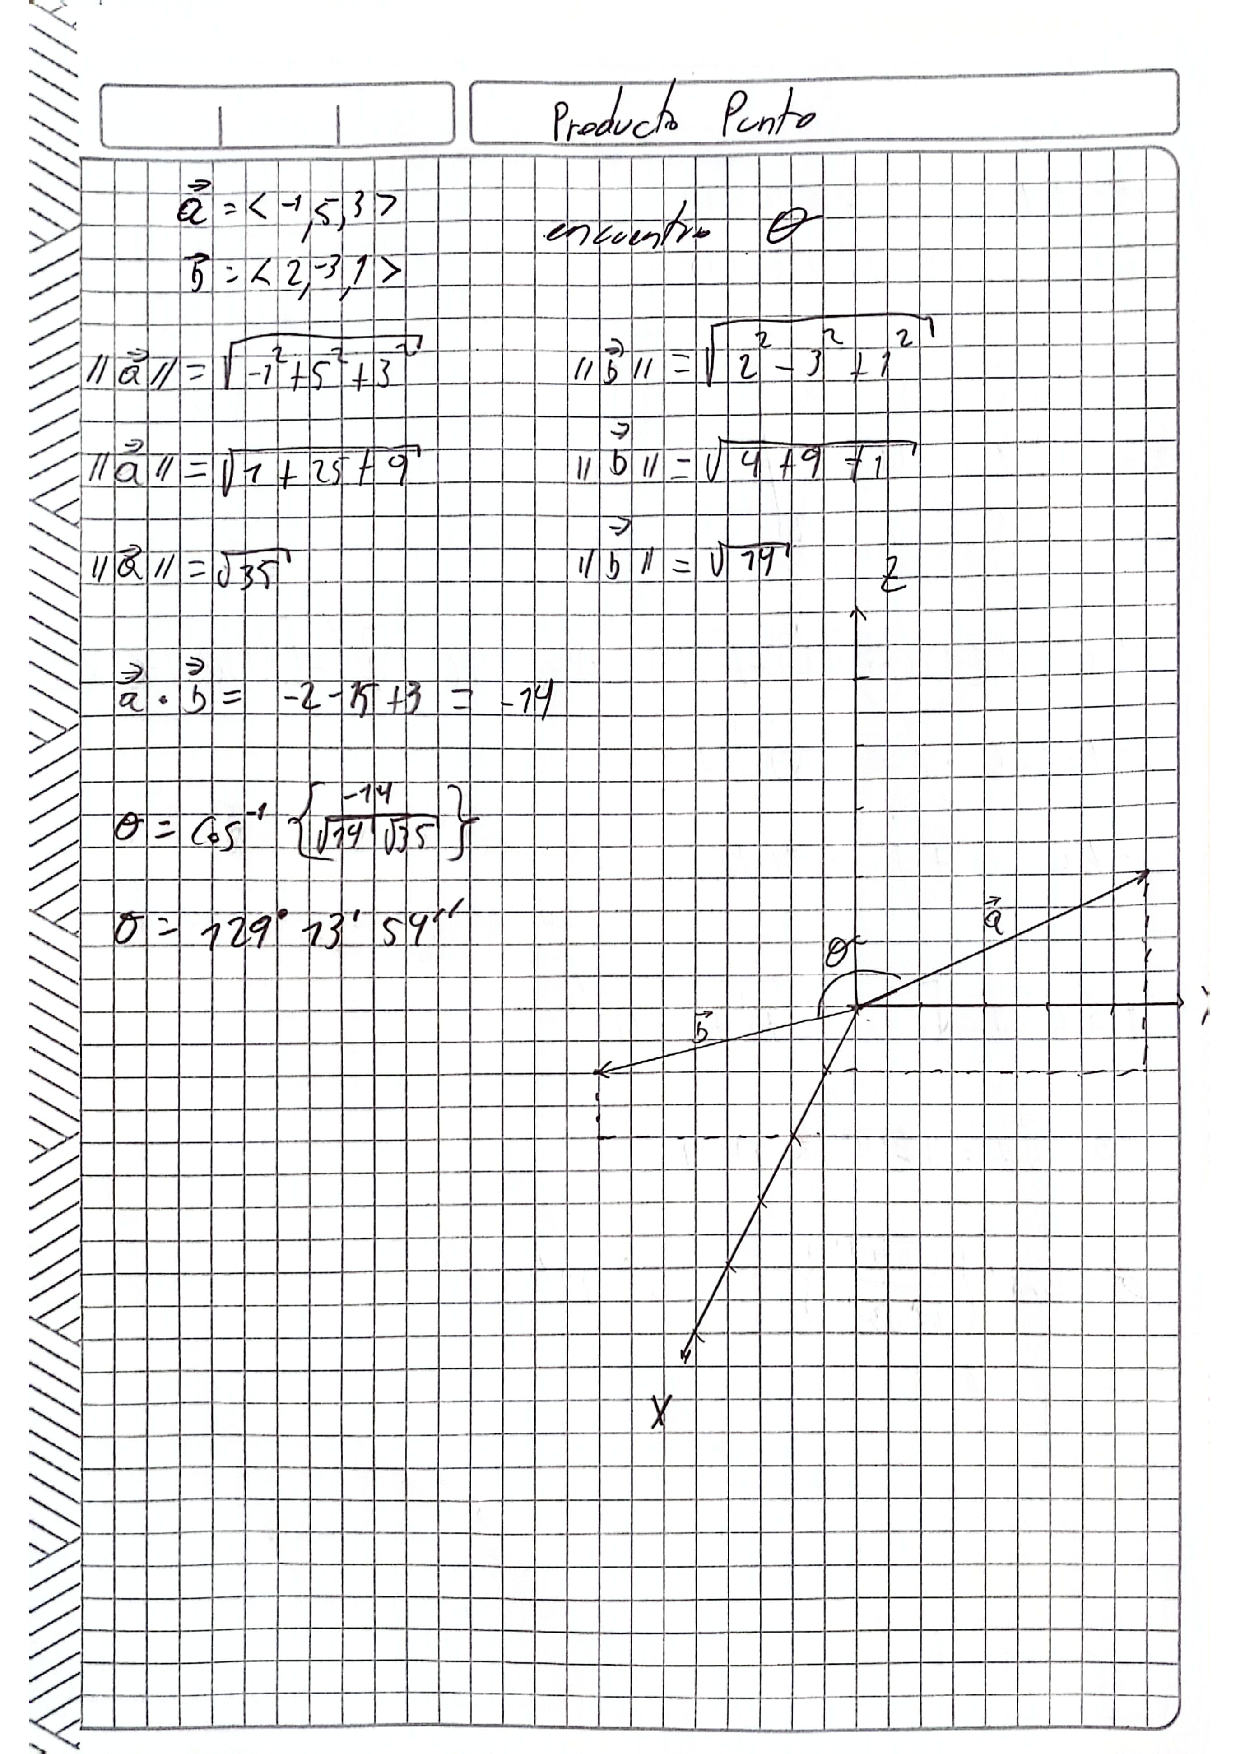
\includegraphics[width=\textwidth]{imgs/Actividad X julio amaya.pdf}
    \end{minipage}
    
    \caption{Izquierda imágenes generadas con GeoGebra y a la derecha los resultados en Python}
\end{figure}

\end{document}
